\section{Experiments}
\todo{Add 2 columns in Table 2}

We have implemented our method in python, utilising the NumPy \cite{numpy}
library for linear algebra operations and the SciPy \cite{scipy} library for an
implementation of \hcluster.
We have used a linkage-matrix \cite{scipy-hcluster-linkage}  based
data structure to store the tree, and have precomputed and cached several
operations that may need to be repeated every refinement iteration. This allows
us to quickly perform the merge and split operations and calculate the
scores (Section \ref{s:refinement}), without having to do (relatively)
expensive tree traversal operations in each iteration of the abstraction
refinement loop. 

Using this implementation, we have performed three sets of experiments to
demonstrate the usefulness of our technique. In several safety critical
settings, such as medical diagnosis and collision detection, where \dnn are
deployed as classifiers, false negative classification with respect to some
classes are highly undesirable. In the first set of experiments, we show that
our abstraction technique can be leverage to obtain effective compression of
\dnn in such settings with a guarantee that the compression does not introduce
any new false negative classifications (Section \ref{s:exp-mnist-comp}). In our
second set of experiments, we demonstrate how our technique may be used to
obtain abstract networks with the aim of proving a given property, plotting the
number of spurious counterexamples introduced as the size of the abstract
network reduces (Section \ref{s:exp-mnist-rob}). Finally, in the last set of
experiments, we show how our technique may be used in a CEGAR loop
\cite{cegar-nn} to verify the \acasxu properties. We utilized \abcrown as the 
solver in the backend for these experiments.



\footnote{The entirety of the code, networks, datasets, and properties utilized in our 
evaluation can be found on \todo{add github link}}.


The experimental results in Tables
\ref{t:acas-verif},\ref{t:mnist-compr-summary} and \ref{t:acas-ncex} were
run on a machine running on an Intel(R) Core(TM) i7-9700K with 8 CPUs running at
3.60GHz, having 16 GB RAM and running Ubuntu 22.04 LTS. The results in
\ref{f:mnist-class} were produced on a machine running on an 
Intel(R) Core(TM) i7-13700 with 24 CPUs running at
5.20GHz, having 32 GB RAM and running Ubuntu 23.10.

\todo{Add details of other experiments}

\subsection{Compression with Guarantees on Critical Classes}
\label{s:exp-mnist-comp}

\todo{ Re-run without re-merging}

In several safety-critical applications of \dnn as classifiers, there are
certain `critical` classes for which a false negative classification is far more
dangerous than a false positive one. For example, for medical diagnosis and
collision detection, a false negative is far more dangerous than a false
positive.

Safety critical analysis of neural networks is highly sensitive to the size of
the network. While several neural network compression techniques exist 
\cite{dnn-compression}, they do not provide formal guarantees 
connecting the behavior of the compressed network and the original network.
Similarly, although existing semantic abstraction techniques have been proposed
as a way to compress neural networks, the guarantees provided by such 
techniques are of an empirical nature \cite{lin-comb-abs-jan}.
This lack of guarantees also limits the usefulness of these compression
techniques as optimisation steps when deploying a network to a
resource-constrained environment. 

Our theoretical framework for abstraction allows us to produce compressed
networks with the formal guarantee that the abstraction process will not
introduce any new false negatives. We do this by marking the output neuron $n_c$
corresponding to the critical class in the output layer as \inc, and all other
neurons in that layer as \dec.  Then, for any input that \cnc classified into
the critical class, $n_c$ will have the largest value in the
output layer, and as it has been marked as \inc, it will continue to have the
largest value in the output layer for \abs as well. Thus, the
abstract network will also classify this input as critical. We will however pay
for this compression by introducing false positives.

We demonstrate the effectiveness of our abstraction method as a
compression-with-guarantees technique via some experiments on \mnist. We set the
class '0'
as the critical class. Then, starting with the fully merged network, we
iteratively perform refinements while measuring the accuracy, false/true
positive/negative rates. We perform this experiments with four strategies of
selecting the culprit neuron $\gamma$ to refine:

\begin{itemize}
    \item \textit{random}: Choose $\gamma$ at random. This serves as a
        baseline.
    \item \textit{samples}: An uniform sampling of the input space is used to
        generate a large set of \gencex $\vct{\beta}$. These are used to
        calculate the score and select $\gamma$ as in 
        \ref{s:refinement}.
    \item \textit{pgd}: The $\vct{\beta}$ are generated via a PGD
        \cite{pgd, pgd-attack} attack on \abs, and then used in a manner similar
        to \textit{samples}.
    \item \textit{samples-pgd}: Initial refinement steps are done following the
        \textit{samples} strategy, switching to \textit{pgd} when all the
        samples have been exhausted.
\end{itemize}

We use the \abcrown implementation for \pgd.

\begin{figure}
    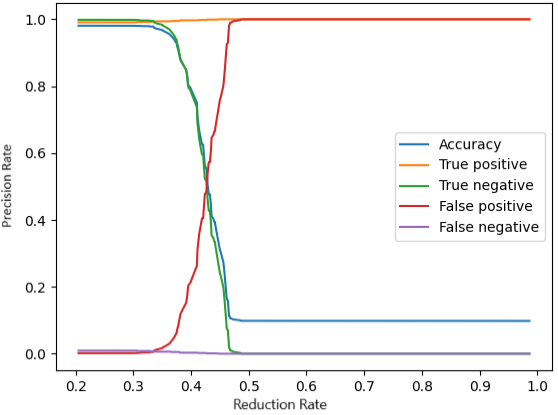
\includegraphics[scale=0.6]{figs/mnist_2_256_compr_pgd-after-samples.png}
    \caption{Accuracy and True/False Positive/Negative Rates vs Reduction Rate
        plot for \mnist of size $2 \times 256$ with critical class 0. Refinement
    done via the \textit{samples-pgd} method. \todo{Add more graphs}}
    \label{f:mnist-class}
\end{figure}

Figure \ref{f:mnist-class} shows some typical plots of the true/false
negative/positive rates (y-axis) against reduction rate (x-axis). Note that the
reduction rate plotted is with respect to the size of the network obtained after
\inc-\dec splitting. While this may mean that \abs produced may be greater in
size than the original network, note that in such an \abs each neuron can be
cleanly classified as \inc or \dec with respect to a property of interest, which
may make formal analysis simpler. Indeed, it has been seen that such \abs, while
larger, may be easier to verify \cite{cegar-nn}.

We notice that, as guaranteed by the theory, the false negative rate never
increases, even as the reduction rate approaches close to $100\%$. In fact, the
false negative rate improves, as some of the points that are going
to be newly classified as positive may in fact be true positives.  
However, as discussed before, we do pay for the compression by introducing false
positives, which we see in the graph. 

We also find in the graph that there is a
small window of reduction rate values where almost all of the improvement in the
false positive rate occurs. This indicates that we eventually are able make 
significant improvements in false positive rate while sacrificing reduction rate
as little as possible. Thus our technique is able to use the semantic
information to order and undo merge operations in an optimal way.

\begin{table}
\begin{tabular}{|c|c|c|c|c|}
\hline
Net Size     & Refinement  & Reduction & Accuracy & Steps  \\ 
\hline
$2\times256$ & random      & 50   \%   & 98.1 \%  &    923 \\ 
$4\times256$ & random      & 50   \%   & 97.6 \%  &   1917 \\ 
$6\times256$ & random      & 50   \%   & 96.9 \%  &   2999 \\ 
$2\times256$ & samples     & 45.7 \%   & 98.0 \%  &    326 \\ 
$4\times256$ & samples     & 40.1 \%   & 95.7 \%  &   1028 \\ 
$6\times256$ & samples     & 45.5 \%   & 96.9 \%  &   2425 \\ 
$2\times256$ & pgd         & 53.4 \%   & 13.7 \%  &     85 \\ 
$4\times256$ & pgd         & 96.9 \%   & 09.8 \%  &      0 \\ 
$6\times256$ & pgd         & 30.6 \%   & 15.1 \%  &   1482 \\ 
$2\times256$ & samples-pgd & 46.0 \%   & 97.8 \%  &    316 \\ 
$4\times256$ & samples-pgd & 40.1 \%   & 95.8 \%  &   1017 \\ 
$6\times256$ & samples-pgd & 45.5 \%   & 96.9 \%  &   2425 \\ 
\hline
\end{tabular}
\caption{Summary of \mnist compression Results \todo{Use Reduction Rate Data}}
\label{t:mnist-compr-summary}
\end{table}

Table \ref{t:mnist-compr-summary} summarises the results from running all the
\mnist compression experiments. For each instance, we report the best reduction
rate achieved for a network whose accuracy was close to the best accuracy seen
throughout the refinement process. Note that we currently do not stop our
refinement loop at the precise point where this network is produced, but may
continue to refine beyond this point.

Firstly, we find that \textit{pgd} performs relatively poorly, with fewer
refinements being performed, producing a low accuracy, small network that has
been merged too much. This is because the \abcrown
implementation of \pgd fails to find a spurious counterexample early on in the
refinement process for these instances, leading to early termination. 

The other instances and methods seem to perform
comparably on the same network in terms of reduction rate and accuracy. This is
evidence for the fact that, regardless of what specific strategy is used to
find $\gamma$ in the refinement process, our framework uses the
semantic information to guide the refinement to reach equally optimal \abs.

Further, we see some difference in the number of steps taken by \textit{random}
and the other methods in finding the abstract network. This indicates that while
the \abs reached may be equally optimal, 
heuristics for finding $\gamma$ indeed
shortens the search for the refined network.

We note that in \cite{cleverest-nn}, an eager PGD-attack before each solver call
has been effectively used to accelerate the CEGAR loop. We do not see such
benefits from using PGD, and instead observe that the global view given by
the large number of samples in the \textit{samples} method performs better.
While the relative performance of \textit{pgd} and \textit{samples} may be
different for a different set of target network and property, our framework
allows the use of either, and in-fact, any other method for generating the
counterexamples.

\subsection{Robustness on \mnist}
\label{s:exp-mnist-rob}
\todo{Change title}

In this section, we explore how well our abstraction refinement process is able
to remove spurious counterexamples. We start with the abstract network and
iteratively perform refinements, measuring the number of spurious
counterexamples at each step. 


\begin{figure}

    \begin{subfigure}{0.475\linewidth}
        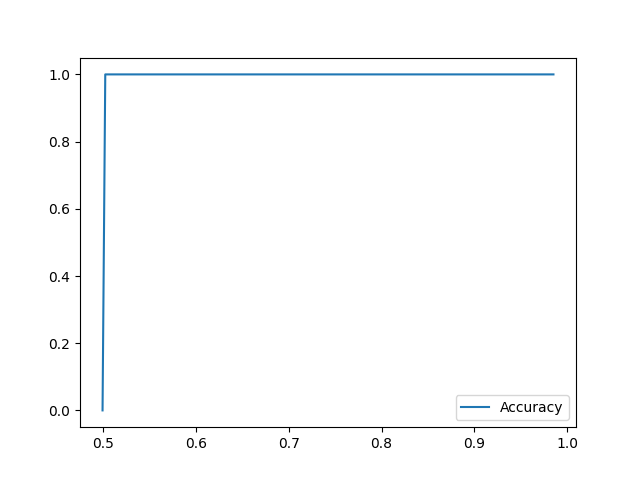
\includegraphics[scale=0.225]{figs/mnist_2_256_prop_0_0.03_samples.png}
        \caption{}
        \label{f:mnist-prop-samples}
    \end{subfigure}
    \begin{subfigure}{0.475\linewidth}
        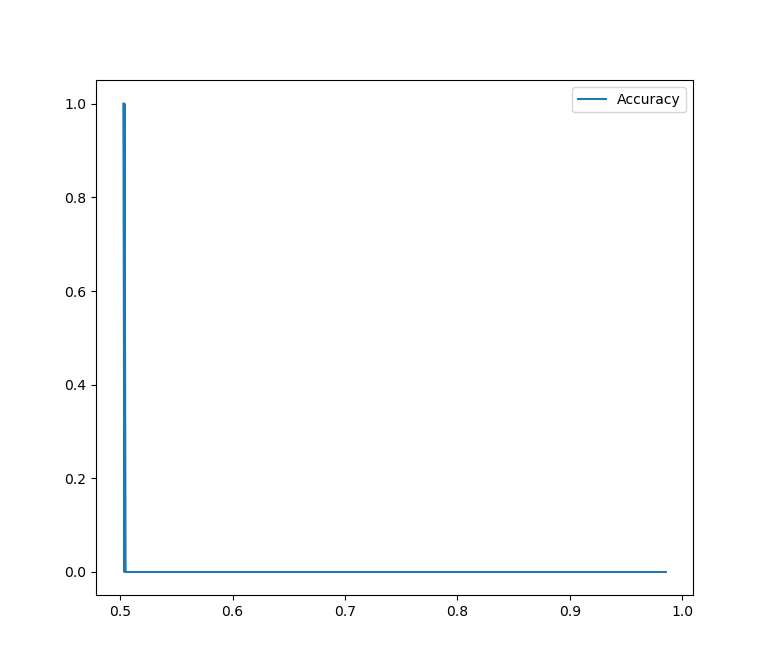
\includegraphics[scale=0.225]{figs/mnist_2_256_prop_0_0.03_pgd.png}
        \caption{}
        \label{f:mnist-prop-pgd}
    \end{subfigure}

    \begin{subfigure}{0.475\linewidth}
        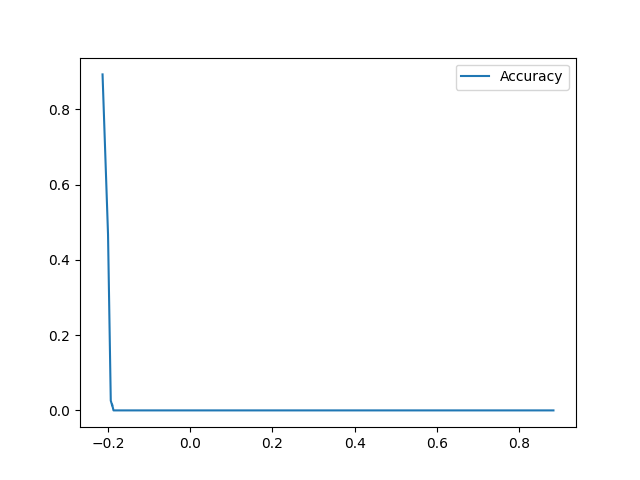
\includegraphics[scale=0.275]{figs/acas_ncex_1_5_4_samples.png}
        \caption{}
        \label{f:acas-ncex-samples}
    \end{subfigure}
    \begin{subfigure}{0.475\linewidth}
        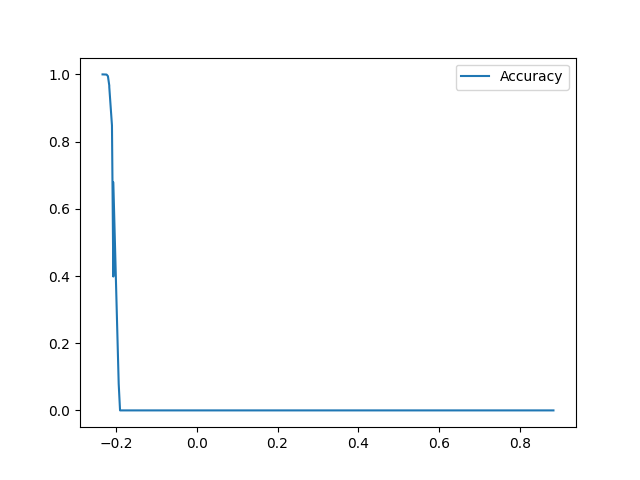
\includegraphics[scale=0.275]{figs/acas_ncex_1_5_4_pgd.png}
        \caption{}
        \label{f:mnist-prop-pgd}
    \end{subfigure}

    \caption{Accuracy vs Reduction Rate plot for \mnist of size $2 \times 256$
        with $\epsilon$-Robustness property. Refinement done via the 'pgd' in
        \ref{f:mnist-prop-pgd} and 'samples' in \ref{f:mnist-prop-samples}
    method. \todo{Make compression rate wrt inc-dec-split size, do 1-current
accuracy.}}
    \label{f:ncex}
\end{figure}

We experimented with two sets of networks and properties: \mnist and \acasxu.
Figure \ref{f:ncex} shows some typical plots
for these experiments. Here the x-axis measures the reduction rate, and the
y-axis one minus the rate of true counterexamples within a random sample - thus
a high value indicates a good abstraction.

 We see that as we refine the
network and the reduction rate reduces (moving right to left along the graph),
the y-value remains close to zero, At some point however, it jumps up
sharply and becomes close to $1$. Thus, we have a small window of reduction rate
values in the graph where we see all the improvement in over-approximation, as
opposed to having a lingering tail of continual improvements as the reduction
rate continues to decrease.
This indicates that, while our refinement process is not able to produce small
improvements in the over-approximation rate, guided by the semantic information
we undo precisely those merges that leads to most improvement in quality while
introducing the least number of neurons.

This indicates that there are a few
critical refinement steps that remove almost all spurious counterexamples. This
may be due the fact that with epsilon robustness properties that are being
explored here, the pre-condition region may be very small, so a single
refinement step may change the behavior of the network on that small region in a
way that eliminates all possible spurious counterexamples from that region.
\todo{Make graphs smaller, and include the vs steps graphs}

\begin{table}
\begin{tabular}{|c|c|c|c|c|}
    \hline
    Net Size     & Refinement  & Reduction & Accuracy & No. Steps \\
    \hline
    $2\times256$ & random      & $49.1\%$  & $100\%$  & $ 809$    \\
    $4\times256$ & random      & $49.6\%$  & $100\%$  & $1778$    \\
    $6\times256$ & random      & $49.7\%$  & $100\%$  & $2602$    \\
    $2\times256$ & samples     & $50.3\%$  & $100\%$  & $  27$    \\
    $4\times256$ & samples     & $49.9\%$  & $100\%$  & $ 648$    \\
    $6\times256$ & samples     & $47.9\%$  & $100\%$  & $1199$    \\
    $2\times256$ & pgd         & $50.4\%$  & $100\%$  & $  28$    \\
    $4\times256$ & pgd         & $88.6\%$  & $  0\%$  & $  14$    \\
    $6\times256$ & pgd         & $83.3\%$  & $  0\%$  & $  82$    \\
    $2\times256$ & samples-pgd & $50.3\%$  & $100\%$  & $  27$    \\
    $4\times256$ & samples-pgd & $49.9\%$  & $100\%$  & $ 648$    \\
    $6\times256$ & samples-pgd & $47.9\%$  & $100\%$  & $1209$    \\
    \hline
\end{tabular}
\caption{Summary of \mnist Results on a single robustness property \todo{Add
        column with time per refine, and number of neurons eliminated per
refine.}}
\label{t:mnist-prop-summary}
\end{table}

Table \ref{t:mnist-prop-summary} summarizes these results for multiple \mnist
networks and multiple refinement methods. Accuracy here refers to the final
accuracy of the best network found when the refinement process stops due to lack
of counterexamples. Firstly, we find that 'pgd' performs poorly on the $4$ and
$6$ layer networks, where while the number of steps are relatively low and the
reduction rate is high, the accuracy is very low. This is because the \abcrown
implementation of \pgd fails to find a spurious counterexample early on in the
refinement process for these instances, leading to early termination without
ever hitting the accuracy jump. 

Apart from these exceptions, the other instances and methods seem to perform
comparably on the same network in terms of reduction rate. This is evidence for
the fact that, within the limited search space of abstractions defined by our
tree, there exists a strong enough abstract network with a good reduction rate,
and that it is possible to find this network via a \cegar-like approach. 

Further, we see significant difference in the number of steps taken by 'random'
and the other methods in finding the abstract network. This indicates that our
heuristics for finding a culprit neuron to base the refinement on indeed
shortens the search for the refined network. We also observe that
'samples','samples-pgd' and for the $2$ layer network 'pgd' take similar number
of refinement steps, indicating that each method may be taking close to the
optimal set of refinement steps. So, although the 'pgd' method
incurs a significant time overhead \dmcmt{Measure?} it does not necessarily
provide any benefits. 

We note that in \cite{cleverest-nn}, an eager pgd-attack before each solver call
has been effectively used to accelerate the CEGAR loop. We do not see such
benefits from using pgd, and instead observe that the global view given by
the large number of samples in the `samples` method performs better. While the
relative performance of `pgd` and `samples` may be different for a different set
of target network and property, our framework allows the use of either, and
in-fact, any other method for generating the counterexamples.

\begin{table}
\begin{tabular}{|c|c|c|c|c|}
\hline
Benchmark         &    Size  & \% Sp. Cex. & Steps   \\
\hline
samples           & 326.878  &  87.0\%     & 294.111  \\
random            & 294.306  &  96.4\%     & 512.011  \\
pgd               & 295.422  &  83.9\%     & 235.606  \\
pgd-after-samples & 329.311  &  94.7\%     & 299.272  \\
\hline
\end{tabular}
\caption{Summary of \acasxu, measuring the percentage of spurious counterexample }
\label{t:acas-ncex}
\end{table}

\subsection{Verification of \acasxu}

\todo{ Talk about the
    fact that if we refine after the first solver call, then we end up refining
all the way.
}

\todo{ Say this: Our fw makes it possible to use the semantic beh to
    unambiguously order refinement operations. Therefore, in a cegar loop
    setting, we are able to make refinement operations precisely until the point
    where the current sp.cex. is eliminated. Prev. techniques needed heuristics
    to guide the refinement order, or chose an arbitrary number of refinement
    steps. Thus, we get fewer solver calls (number) , and between each each call
    we are making precisely the right number of refinemets in an order optimal
    wrt sem.info.
}

In these set of experiments, we have taken the \acasxu set of
networks \todo{add detailed table} and
properties and attempt to verify them using a \cegar approach. We use our
technique to generate the abstraction, and attempt to verify the property on the
abstract network using an existing neural network verification solver. If the
solver returns a counterexample, and if that counterexample is not spurious, we
use that counterexample as a reference point for score calculation  to select
the culprit neuron (\ref{s:refinement}). With the culprit neuron selected, we
then refine the network.

\begin{table}
\footnotesize
\begin{tabular}{ |c|c|c|c|c|c| }
\hline
Benchmark   & \% Verified & Size     & Time    & No. Refine & Solver Calls \\ 
\hline
prop-Safe   &   64\%      & 339      & 11.1    & 302        & 5.8      \\
prop-Unsafe &   93\%      & 140      & 10.0    & 137        & 2.8      \\
adv-unsafe  &  100\%      & 18       & 1.2     & -          & -        \\
\hline                                                                
\end{tabular}
\caption{Summary of \acasxu verification }
\label{t:acas-verif}
\end{table}

The results are summarised in table \ref{t:acas-verif}. The solver we used was
\abcrown. The average times reported here do not include instances where the
verification failed due to timeout, and the reduction rate is with respect to
the network size after inc-dec split. We report these figures since, as noted in
\cite{cegar-nn}, the networks obtained after inc-dec split, while larger, are
easier to verify by typical solvers like \marabou.

We notice that for the unsafe cases, we are able to refute the
properties via a counterexample obtained on a significantly smaller network. In
fact, for most networks, we are able to refute based on a counterexample from
the fully abstracted network of size $18$ (See \todo{Add ref to full table in
appendix after re-runs}. Note that since we use only two classes in our
fully abstracted network as opposed to 4 in \cite{cegar-nn}, the size of this
network is significantly smaller. 

For safe cases, we see only negligible improvement in the size of the network.
We believe that this is because for these benchmarks, there is not much room for
improvement via abstraction. We are also able to only verify a smaller
percentage of these benchmarks, because the underlying solver call would time
out on mid-sized abstract networks \todo{Ref full table in appendix}, stalling
the CEGAR loop. We note that some timeouts were also reported in
\cite{cegar-nn}, and thus may be expected. 

In our experiments we find that the time taken for a solver call are more
dependent on the particular solver, solver configuration and benchmark than on
the size of the network. Thus it may seem that the effort needed to verify a
network is dependent on other factors than simply the size of the network. While
this may be interesting to explore in future work, we nonetheless argue that
network size is a relevant metric. This is as more and more solvers are designed
and optimized for various kinds of networks, the underlying worst case
performance will almost certainly remain exponential in the size of the network.
Furthermore, in the previous experiments (Sections \ref{s:exp-mnist-comp},
\ref{s:exp-mnist-rob}) we have demonstrated that our abstraction technique does
produce a reduction in network size whose usefulness extends beyond improving
verification time. 

